\chapter{系统验证实验与性能测试}

上一章节介绍了面诊系统的系统设计与交互设计,本章将介绍对日常可用性和系统可解释交互设计进行的实验设计及实验结果,最后介绍对系统的基本性能测试及结果。

\section{实验1:日常可用性实验设计与验证}

\subsection{实验设计}
为了验证本文设计的交互界面的有效性,本文设计了一个交互验证实验,用于验证客户端的实现是否解决了交互的可用性问题。

\begin{figure}[h]
    \centering
    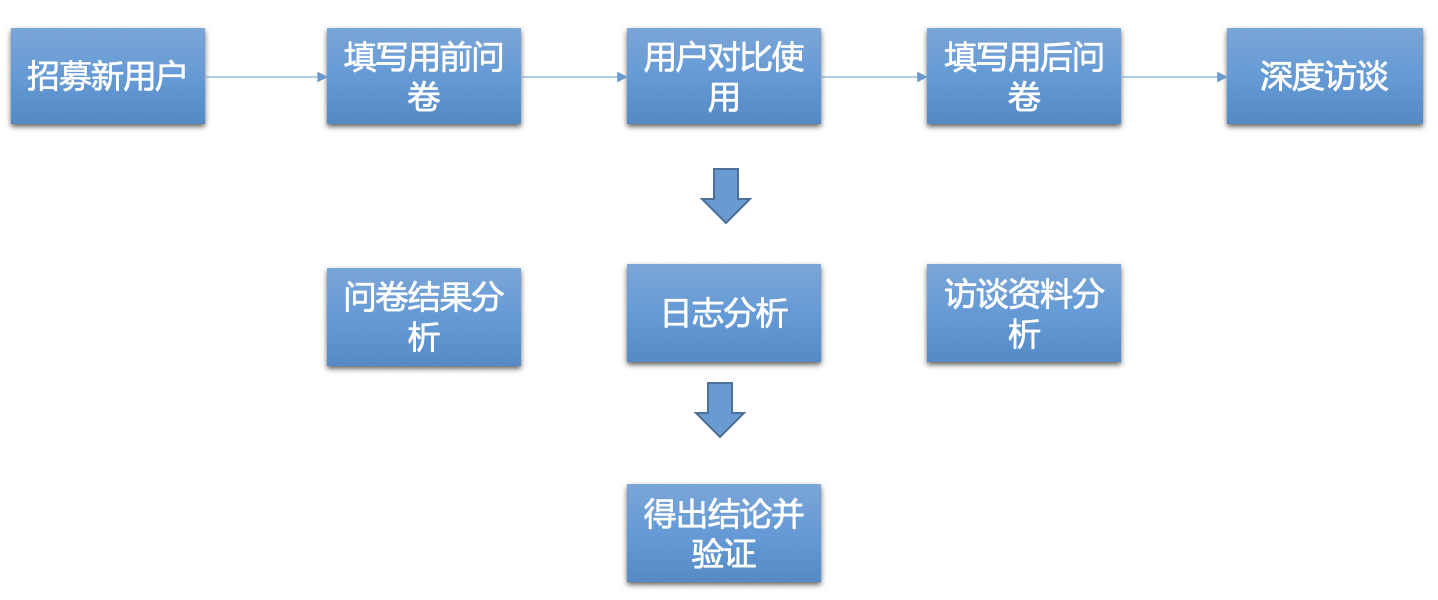
\includegraphics[width=15cm]{images/exp.png}
    \caption{实验设计}
    \label{fig:exp}
\end{figure}

如图\ref{fig:exp}所示,实验流程如下:
\begin{enumerate}

    \item 通过海报(如图\ref{fig:poster}所示,具体内容有对应的修改)和社交媒体,招募到了12位对中医感兴趣的志愿者参与了本次实验。

    \item 在招募到志愿者之后,本文通过面诊系统的问卷关联功能,让每个用户填写一个志愿者的基本信息的问卷,然后单独给每位志愿者介绍这次实验的背景和这次实验的整个流程。

    \item 通知用户回家自由使用,本文可以通过面诊系统的用户操作记录管理功能观察用户的使用日志,实验期间用户也可以随时反馈使用感受。

    \item 用户持续使用了大概两周之后,单独对每位用户进行深度访谈,通过录音的方式记录访谈数据。

\end{enumerate}

\subsection{实验结果}


% \begin{figure}[ht]
%     \centering
%     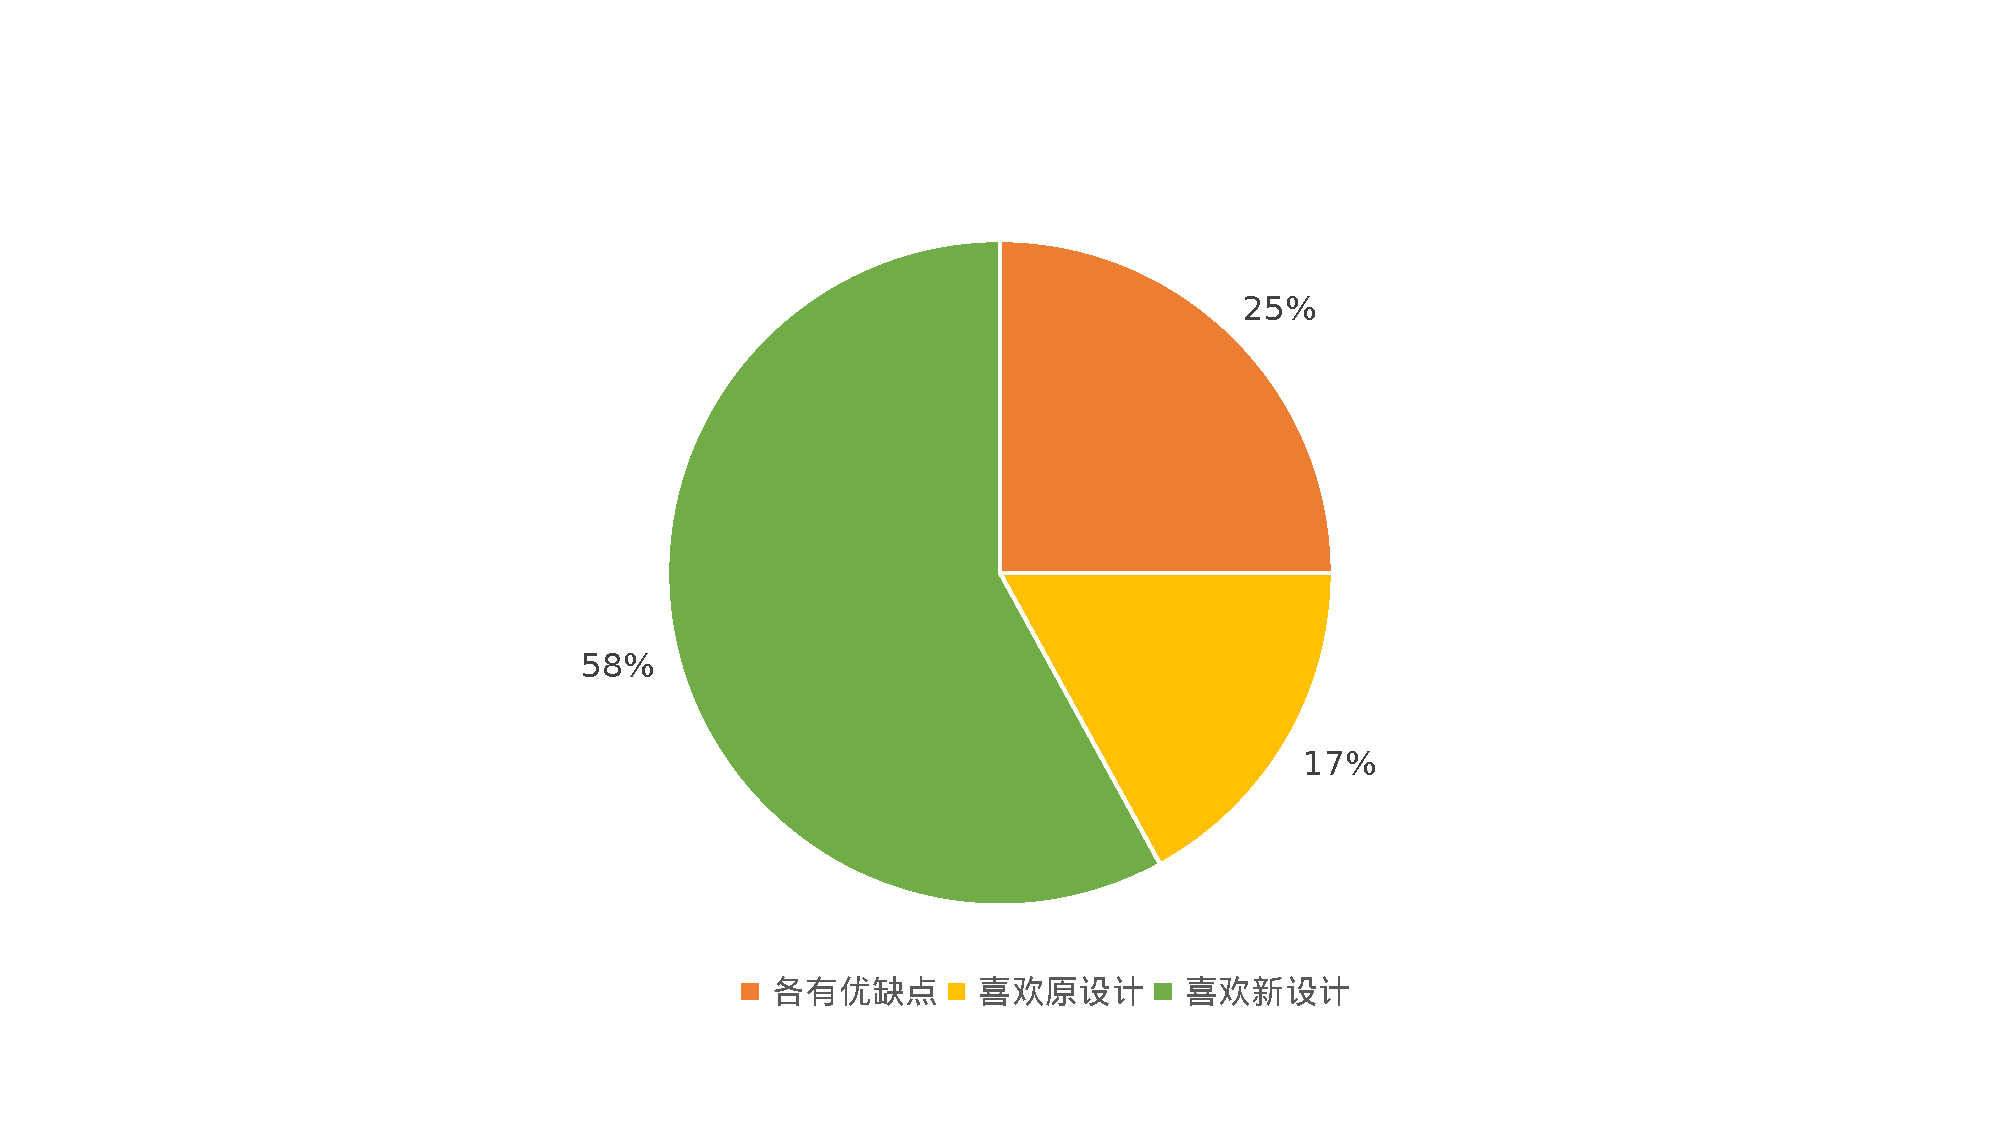
\includegraphics[height=8cm]{images/ui-exp.pdf}
%     \caption{界面设计实验结果}
%     \label{fig:ui-exp}
% \end{figure}

有少量志愿者选择持续使用原设计完成诊断,大部分用户选择本文的新设计并且原因与用户研究中的结果一致,而剩下部分用户觉得两种设计各有优缺点,具体原因如下:


\subsubsection{选择新设计}

和之前的用户研究的结果类似,新设计的确能够解决用户的部分日常可用性问题。

根据访谈数据,其中一位参与者认为新设计可以让他在日常使用时只完成自己想做的部分,更加方便:
\myfont{新设计方便,单独做某一块检测;给的指示不空洞;有针对性和选择性。}、\myfont{设计挺好的,感觉更方便一些。}

如预期,新设计带来的可选择性同样在参与者的身上得到了反馈:
\myfont{新设计诊断透彻到位;可以选择性地做诊断,知道健康得分的构成,帮助了解中医知识,省时间。}、
\myfont{新设计操作更简单,有选择性,但是问诊 的选项太少,涵盖不全。}

另一部分参与者虽然觉得新设计不好看,但是相对于原先缺乏可用性的设计,新设计基本解决了他的问题:
\myfont{虽然新设计界面丑,但原设计问诊很烦,而且新设计能实时显示舌诊结果。}、\myfont{想按照顺序回答问卷,新设计问诊界面不舒服;但是新设计的选择性检测比较方便。}


\subsubsection{选择原设计}
虽然新设计的设计理念是为了方便用户的持续使用,但也同样增加了界面的复杂度。

在选择使用原设计版本的用户中,其中一位参与者就认为新的设计对于他没有帮助而更倾向于一开始有模拟传统中医面诊流程感(先面诊舌诊再问诊)的原设计版本:\myfont{原设计界面好看,问诊流程有完成感,并不想知道具体的症状对应什么细节。}而另一位参与者则认为问诊应该一次性全部完成,这样在操作上感觉更加连贯:\myfont{原界面设计更符合常规,问诊是连贯的,首页内容很清楚。}

本文提出的设计,虽然能够简化用户的操作,但是会让用户失去自己完成诊断的流程感。
新设计选择了一次性展示用户上次的诊断结果,但是本文的设计在内容丰富度和简单性的取舍下,选择了没有显示原有的问题和所有的选项,用户反馈这种代替用户做选择的方式让用户觉得没有参与感。
当用户希望得到更加准确的面诊结果的时候,繁琐的操作是可以忍受的。

\subsubsection{各有优缺点}
部分用户在实验过程中,两个设计的版本都在交替使用,也难以确定哪一个版本更加合适:
\myfont{界面设计更符合常规,问诊是连贯的,首页内容很清楚;新设计圆圈里的不同颜色有提示功能。}、
也有部分参与者反馈新设计并没有符合本文设计的预期,一次性展示所有的选项同样会让用户觉得所有的选项都必须选择:
\myfont{想按照顺序回答问卷,新设计问诊界面不舒服;但是新设计的选择性检测比较方便。}、
\myfont{新设计更方便,但一个一个问题点开很烦;原设计流程顺利,简单。}

\subsubsection{操作耗时对比}

\begin{figure}[ht]
    \centering
    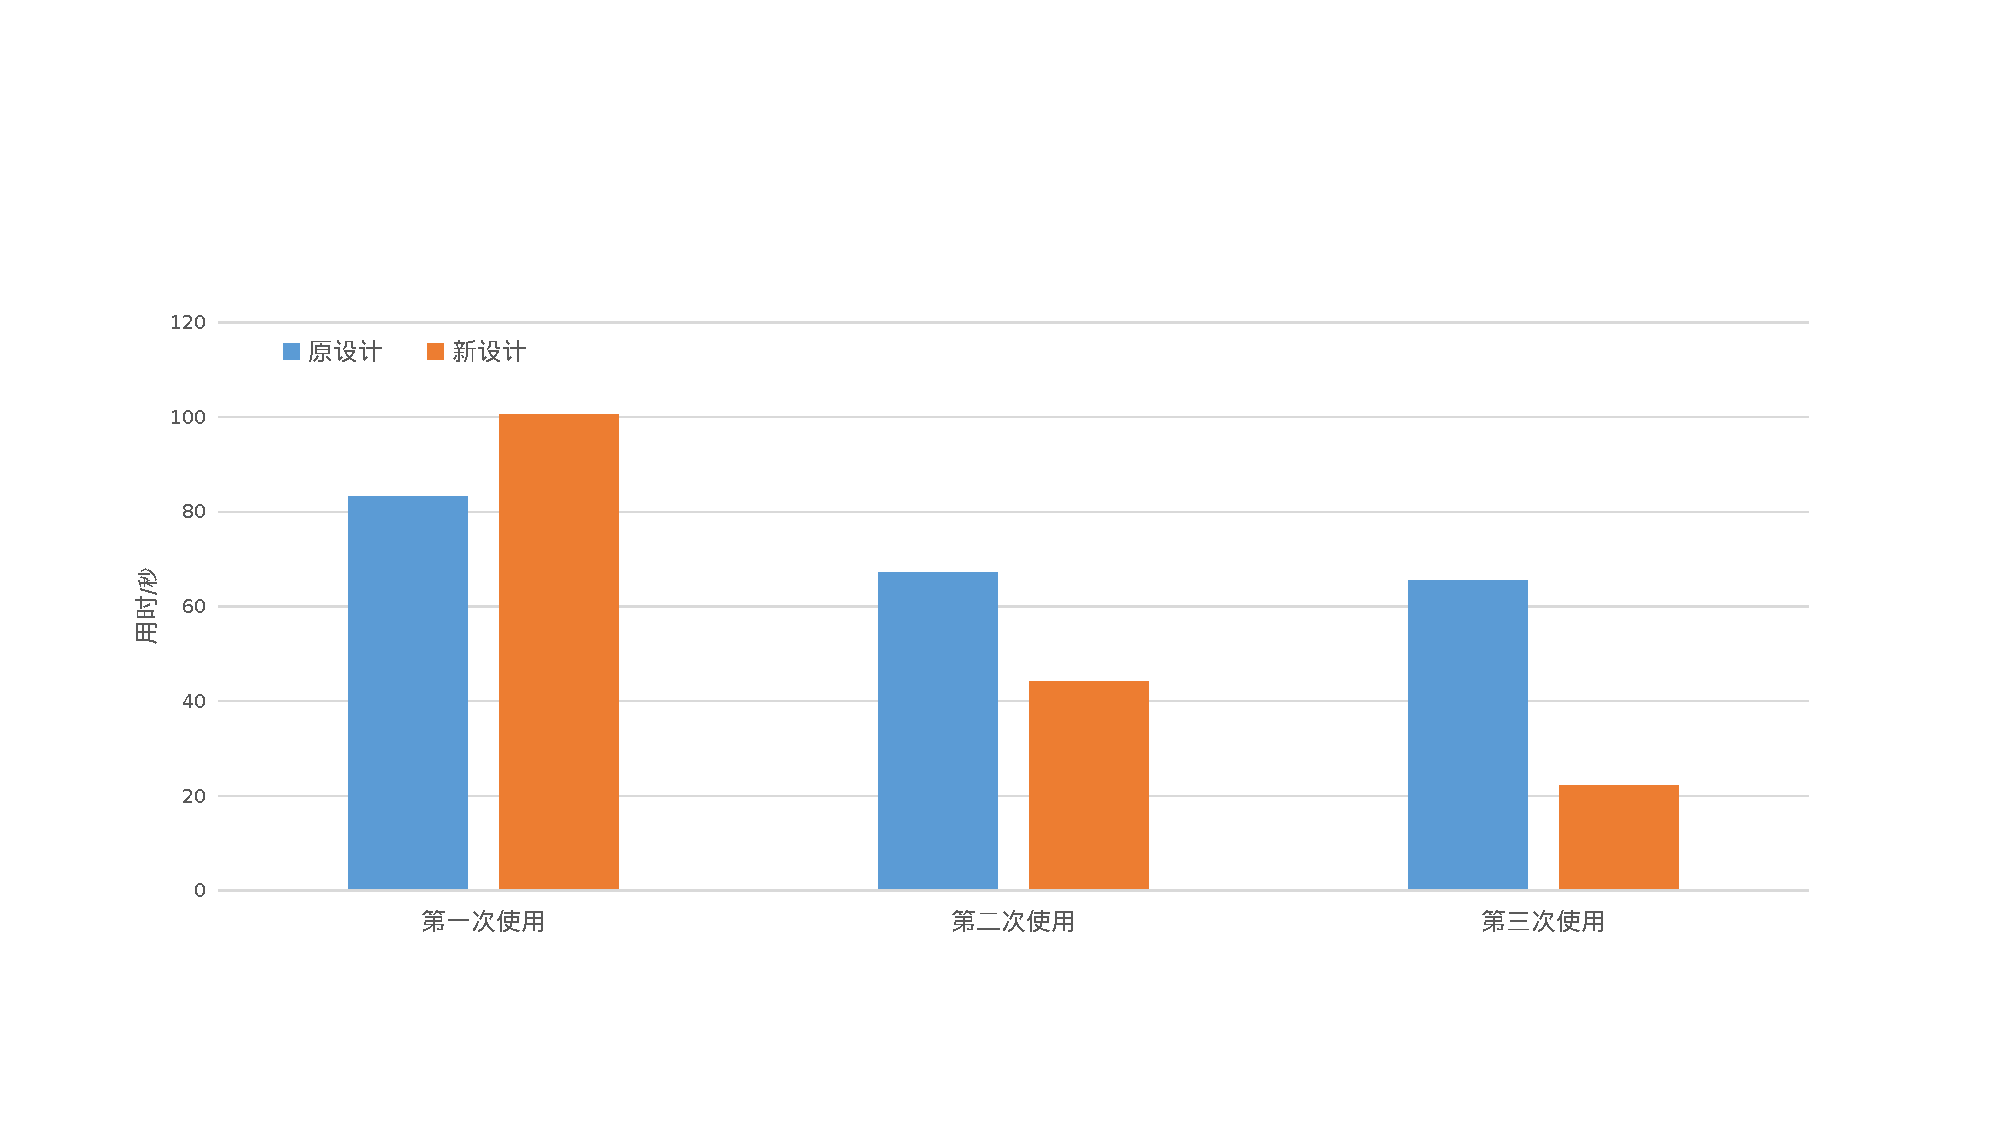
\includegraphics[width=13cm]{images/time.pdf}
    \caption{操作耗时}
    \label{fig:ui-time}
\end{figure}

由于大部分参与者在实验过程中使用系统进行诊断的次数不多,因此本文只通过部分用户的操作日志统计了前三次从进入诊断页面到完成诊断的时间,数据经过处理后的结果下:
\begin{itemize}

    \item 第一次完成面诊的操作耗时,新设计相比原设计对于用户来说需要更长的时间。如之前的参与者的反馈,新设计没有原设计直观和简单,由于界面相对复杂,因此用户理解后顺利完成诊断需要的时间也比较长。

    \item 在后续的第二次、第三次操作中,旧设计的操作时间在用户熟悉之后稍有降低,但是总体来说变化不大;新设计可以让用户直观的看到自己上次的面诊舌诊数据和问诊的选择,用户可以只选择完成有变化的部分实现快速诊断,完成一次操作时间大大降低。

\end{itemize}

\subsubsection{总结}
通过实验,本文发现新的设计在一定程度上的确解决了本文在之前提到的可用性问题。用户在日常使用的情况下能减少用户在完成诊断操作上花费的时间。
不过值得注意的是也有部分年纪较大的用户反馈新的设计过于复杂。总体来说符合日常可用性设计策略的预期,能够满足用户日常使用的需要。
% 没有依次做完面诊、舌诊、问诊的完成感,没有做到兼顾所有用户的需求。

\section{实验2:系统可解释性实验设计与验证}


\subsection{实验设计}

为了研究如何对面诊系统进行解释,本文设计了一个交互实现,通过线上实验结合深度访谈的形式进行。

\subsubsection{线上实验}
通过在各大社交平台发布海报,以及使用问卷星的样本服务招募志愿者,经过筛选之后,一共招募了60位左右的用户。

每个用户的实验流程如下:
(1)用户通过扫描二维码,或者通过给定的链接,进入问卷星的调查问卷。
(2) 完成调查问卷之后,跳转到面诊系统。通过调用问卷星提供的企业用户接口,同时把问卷星的问卷id通过ssojump传给系统。
通过ssojump中的问卷id,完成自动登陆,登陆的用户id为wjx-{问卷星id}。
(3) 在用户完成一次面诊之后,会在健康诊断页面下,看到一个跳转链接,可以选择填写用后问卷。其中用前与用后问卷如图\ref{fig:wenjuan}所示,包含量化理解程度的指标和判断对健康知识理解的问题。

\begin{figure}[ht]
    \centering
    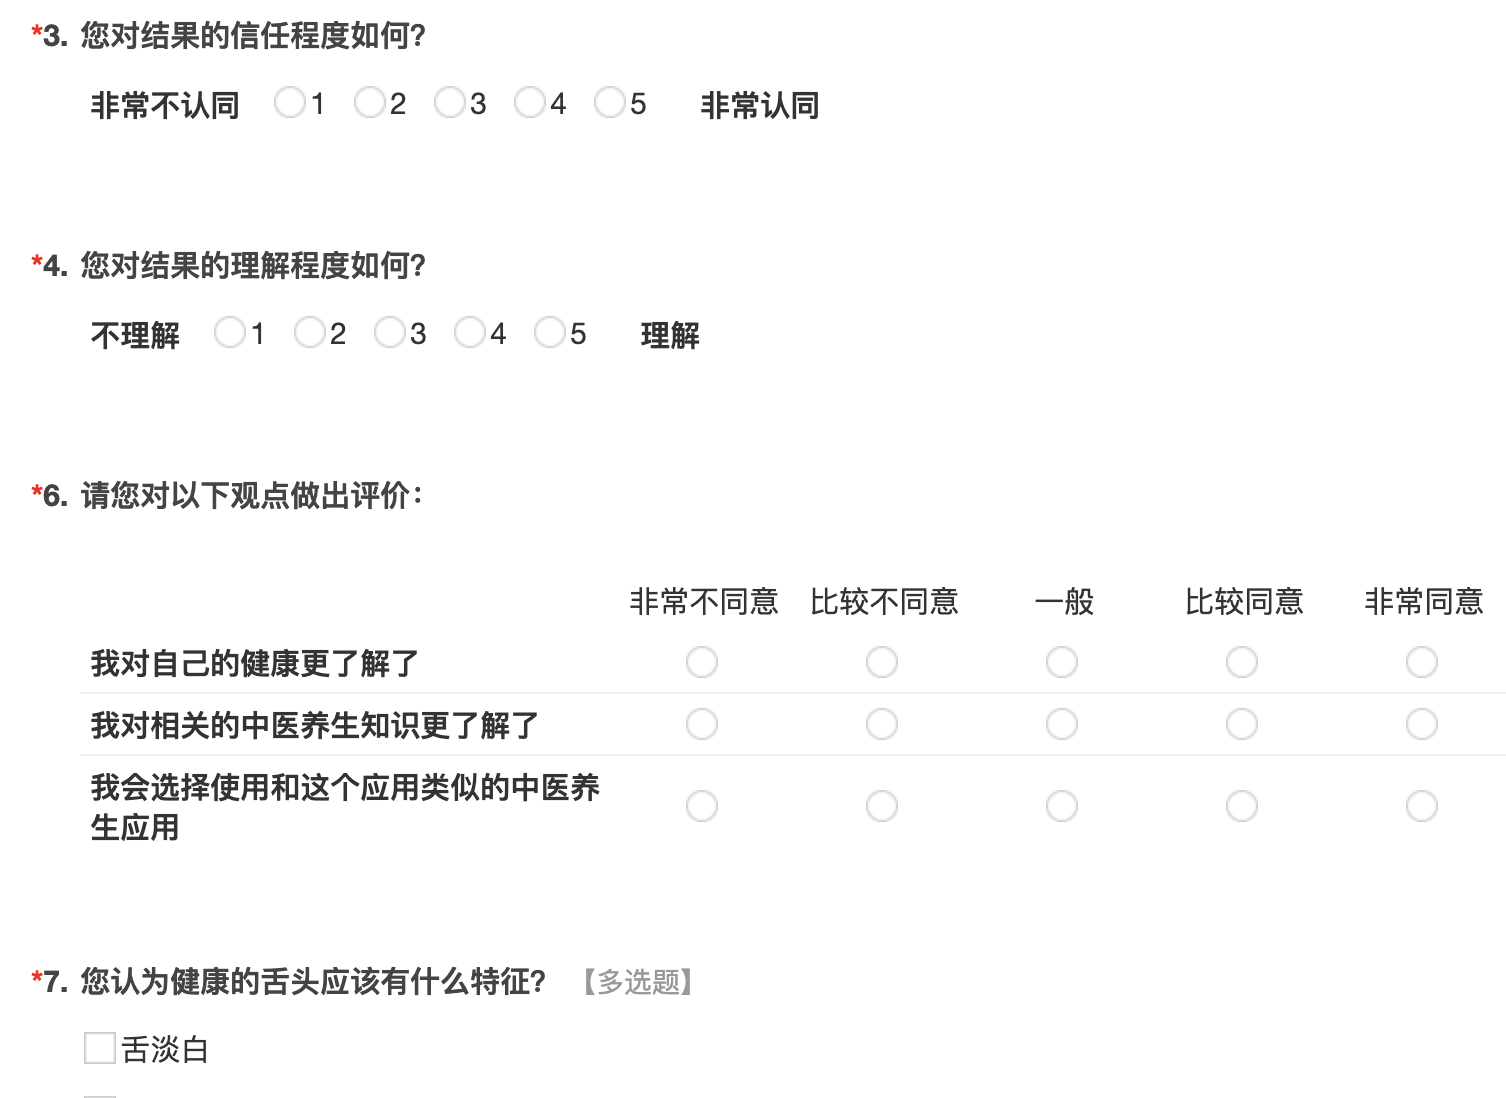
\includegraphics[width=10cm]{images/wenjuan.png}
    \caption{调查问卷}
    \label{fig:wenjuan}
\end{figure}

在实验过程中,用户会被随机分配到有解释的设计和无解释的设计。

\subsubsection{深度访谈}
通过对比,本文发现几乎所有的用户都更倾向于选择添加了解释的系统且提高了对结果的理解。
但定量的数据分析,本文无法得出哪些因变量如对结果的信任与是否有解释的相关性。为了继续研究解释的影响,同时理解为什么实验数据会呈现上述的特点,本文补充了一次深度访谈。

本次实验,本文同样实现了一个可解释的交互设计,界面和流程与上一个实验完全相同,但是去掉了用户登录时的随机分配用户角色,而是添加了一个开关。
当开关关闭的时候,系统不会对结果进行解释;当开关打开的时候,系统会对诊断过程和诊断结果进行详细的解释。

在使用过程中,本文首先让用户试用有解释或者没有解释的版本,鼓励用户在使用过程中随时自己内心的想法。然后通过切换开关,让用户再一次使用。最后对用户进行一次深度访谈。

% \subsection{实验数据}
% 每个用户在参与实验之后,可以得到调查问卷的数据,系统的使用日志,已经用后问卷的数据。

% \subsubsection{可用数据}
% 本次实验可分析的数据来自调查问卷,用后问卷和面诊系统的日志三个数据表,对应的可用数据如下:
% \begin{itemize}
%     \item 调查问卷:序号、提交答卷时间、所用时间、来源、来源详情、IP、个人信息、我相信中医养生、了解中医养生、平时注重养生、经常去看中医、希望自己的生活方式更健康、对学习相关中医养生知识感兴趣、认为中医面诊可以了解健康情况、认为中医舌诊可以了解健康情况、认为智能系统可以自动评估健康情况、随机顺序的中医知识问题。
%     其中个人信息包括性别、年龄段、受教育水平、职业、城市、健康状态等。
%     \item 用后问卷:序号、提交答卷时间、所用时间、来源、来源详情、IP、诊断结果、结果的信任程度、对结果的理解程度、是否愿意使用类似应用、随机顺序的中医知识问题。
%     \item 用户使用日志:序号、用户名、设备信息、操作名、操作信息、日期。
% \end{itemize}


% \subsubsection{信息提取}
% 对于同一个用户在一次实验过程中,若调查问卷的ssojump参数为ID,则此次用户操作记录的用户名为wjx-ID,用户问卷的来源详情为wjx-ID。
% 通过这个对应关系,本文可以利用面诊系统提供的问卷关联的功能,把三个表的信息,合并到一个表中,面诊系统通过表格插件导出下载,最终得到特征如表\ref{tab:exp_data}所示。


% \begin{table}[h]
%     \centering
%     \caption{实验数据汇总}
%     \begin{tabular}{ll}
%         \toprule
%         字段 & 描述 \\ 
%         \midrule
%         序号 & 调查问卷序号 \\
%         性别 & 男/女/未知 \\
%         教育程度 & 本科以下/本科/本科以上 \\
%         工作类型 & 计算机相关/计算机不相关 \\
%         用户类型 & 解释/不解释 \\
%         健康得分 & 探针给出的分数 0-100 \\
%         信任 & 对结果的信任程度 1-5 \\
%         理解 & 对结果的理解程度 1-5 \\
%         前健康知识得分 & 使用探针之前的健康知识得分 \\
%         后健康知识得分 & 使用探针之后的健康知识得分 \\
%         查看了哪些解释 & 使用过程中查看的解释类型 \\
%         \bottomrule
%     \end{tabular}
%     \label{tab:exp_data}
% \end{table}

% 经过处理之后,本文最终得到的数据图表\ref{tab:exp_data}所示,对应的字段说明如下:
% \begin{itemize}
%   \item 工作类型: 根据调查问卷的数据,用户自由填写的职业类型有很多,为了便于分析,本文把 IT经理、IT软件设计、hr、it、互联网、技术研发、技术研发人员、技术经理、电脑工程师、研发、科研、程序员、计算机、软件工程师、软件开发工程师、通信、通讯等归为it相关。

%   \item  信任、理解: 这两个字段来自用后问卷调查表,取值范围为1-5的整数。

%   \item  健康知识得分: 使用探针前后的健康知识得分,使用的是用户回答正确中医知识的个数。

%   \item  用户类型:用户使用的版本,包括原始版本或者添加了解释的版本。

%   \item  查看了哪些解释: 通过检索日志中关键字获取用户查看了哪些解释,其中解释类型包括面诊过程、舌诊过程、体质术语介绍、面诊结果、舌诊结果、健康分数、体质、分数计算公式等。
% \end{itemize}

\subsection{实验结果}

\subsubsection{影响权重的解释方式}
在面诊舌诊和问诊中,都会涉及到本项的诊断对最终体质影响的权重。本文通过实验发现相对于柱状图的方式,雷达图更加适合该场景。

在权重解释这部分,用户不仅可以看到自己目前的舌相或者面相对应的特征,还能看到对每个体质影响的权重,该设计将最后诊断的规则系统部分规则暴露给了用户。
向用户解释这个权重的时候,本文使用了图表的方式向用户解释权重。如图\ref{fig:question_weight}所示,实验迭代的过程中本文先后实现了使用柱状图和雷达图的方式来展示权重。

\begin{figure}[htbp]
    \centering
    \subfigure[柱状图方式]{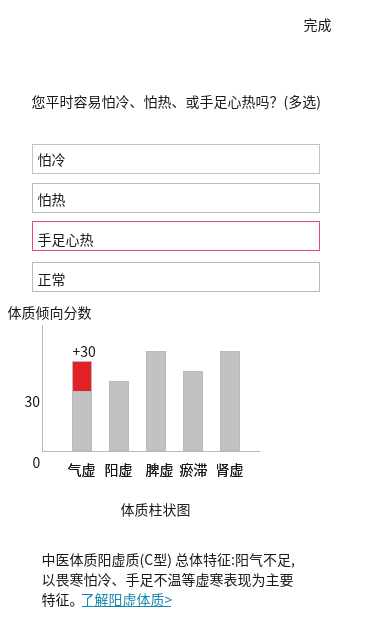
\includegraphics[height=10cm]{images/old3.png}}
    \subfigure[雷达图方式]{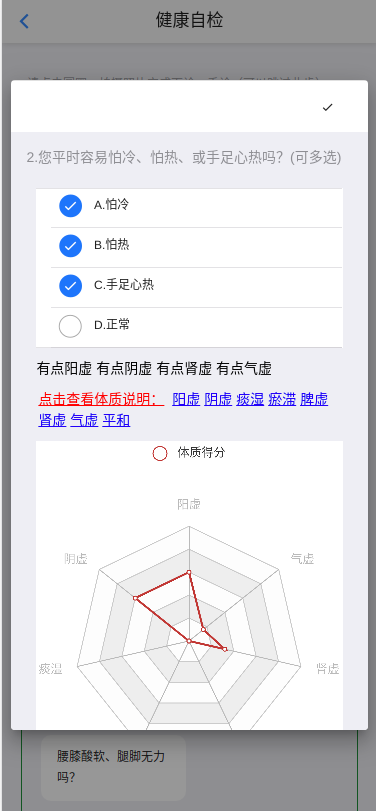
\includegraphics[height=10cm]{images/questions2.png}}
    \caption{影响权重的解释}
    \label{fig:question_weight}
\end{figure}

如图\ref{fig:question_weight}(a)所示,本文在设计中采用柱状图的方式向用户解释该问题对体质倾向影响的权重,其中通过红色突出显示本次出现变化的部分。
但是在实验过程中,经过用户反馈,本文发现在和用户自己健康相关的场景下,柱状图不适合用来解释影响权重。
柱状图在权重差距较大的情况下可能会有一部分\myfont{突出}的比较高,有一个明显的缺点就是柱状图容易引起用户对自己身体情况的焦虑感。部分用户的反馈如下:
\myfont{然后他那个柱状图是太让人心慌了,那么片面的每道题给你一个那么高的值}、
\myfont{下面那个柱状图非常吓人的,弹出来很高,让我有一种我的脾脏已经不行了的感觉}

为了避免在解释影响权重过程中引起用户不必要的恐慌,本系统需要一种相``温和''的方式对影响权重进行解释,于是最终选用了雷达图的方式来解释影响权重。
如图\ref{fig:question_weight}(b)所示,雷达图从外观上来看会让数值的峰值不那么明显。

\subsubsection{日志分析结果}

通过对在线实验数据变量间的相关性分析,结果并没有体现出各个变量和是否看了解释的有强相关性,当前的解释方式对用户吸引力还不够。

根据日志数据,发现本次实验数据中,大多数参与者的完成质量非常差,具体有以下几个特点:
\begin{enumerate}
    \item 虽然本文在线上收集数据的时候,过滤了完成实验用时较短的样本,但是整体的完成实验的时间也是偏短,说明用户在填写问卷的时候没有认真思考。

    \item 日志数据中用户点击了解释的比例不到1/3,点了解释的用户中大部分也只点了面诊、舌诊、体质、结果解释中的一种,剩下的大部分用户并没有去点击去查看解释。
\end{enumerate}

\subsubsection{深度访谈结果}

通过深度访谈,本文发现日常面诊环境下几乎所有的用户都更倾向于选择添加了解释的版本的原因:\myfont{因为第一个版本其实和第二个版本得出来的诊断结果是一样的,它并不会说给我分数提高让我感觉更健康了,它只是说让我看清楚到底是什么问题,我觉得对我来说我是更喜欢第二个版本}、
\myfont{喜欢有解释的,因为它有详细的解释啊。因为可以直接看到你的问题所在,就是可以解释这个症状对应什么问题。}在验证了系统设计有效性的同时,本文发现添加可解释性的影响有以下结论:

\begin{itemize}
\item \textbf{忽略解释的原因}
\end{itemize}

1. 文字提示的形式不明显,不知道可以点击。

参与者被问到为什么没有点开解释查看时,他们的回答是:\myfont{直接看到图形界面了,没有注意到有文字解释}、\myfont{感觉文字不像是可以点的}、\myfont{对,不是很明显,我没注意}、\myfont{好像不太明显,因为我一开始以为是一个什么东西,注意力都在面诊}。
有参与者建议可以做成消息提醒的小红点的形式,利用用户的“强迫症”心理,吸引用户打开解释。

2. 看到解释的提示,但是自己对结果没有疑惑。

两位参与者明确表示自己看到了解释,但是就是没有点,其中一位说道:\myfont{我觉得并不是说你所有的有显示可以点,我就一定要点。}另一位参与者则表示:\myfont{你像面白无光泽,就很直白的这个意思,我就能理解,为什么还要点进去看无光泽是什么意思?}


3. 想尽快完成本地诊断的流程。

另外一个让用户忽略设计中解释的原因是因为本次实验设置的实验流程过于繁琐,部分用户想尽快结束实验的流程,其中一位参与者解释说:\myfont{因为我想快点结束。}
另一位参与者也看到了解释,但是并没有选择点开:\myfont{我不会想去打开,因为我想要做下一题。}

\begin{itemize}
    \item \textbf{提高用户对诊断结果的接受程度}
\end{itemize}


1. 用户知道背后的原理之后,如果结果不符合自己的预期,会尝试从自己方面的原因解释为什么不是这个结果。

当采访者知道自己的个人判断和系统给出的不一致时,他的第一反应是对于自己的判断产生怀疑而不是质疑系统给出的结果:\myfont{问题在我们吧,我也不知道。}而其他的参与者在之后其背后原理之后,也表示对系统的错误可以接受:
\myfont{但你如果你说列出来三个可能的结果,你说你都有这三种结果都有可能。我觉得这种我是可以去接受,里面如果有某一个和我的匹配就行了}、
\myfont{深度学习模型尽管它可能它训练的效果可能没有很完善,但是你加了模型进去以后,它确实是能反映出来个人健康一定的问题。}


2. 提高对错误结果的接受程度。

在参与者知道深度学习需要大量的数据后,即使当前结果不太符合预期,也能理解目前数据量可能不足,有一定的错误率是正常的:
\myfont{也不能说完全不能接受,就像你前面也说了,他说根据大数据样本去得出来的,而且但这个可能并不符合每个人的情况很正常。}、
\myfont{等训练数据足够大了也许效果就会好很多。}

\begin{itemize}
    \item \textbf{增加对系统的信赖程度}
\end{itemize}

参访者认为系统用到了实际的深度学习的技术, 觉得更加可信赖:\myfont{但是你加了一个是深度学习模型进去,不管怎么样,它至少用到了一定的科学技术。}
另一位采访者觉得因为研发的机构比较权威,系统比较可靠:\myfont{我信当然信,你不觉得人们很容易有这种名牌效应,觉得牌子在这放着就不错。},而另一个参与者在知道本系统用到了中医药大学提供的诊断规则之后也表示:\myfont{我觉得你们比较权威。}

\begin{itemize}
    \item \textbf{对于提高中医的理解的帮助}
\end{itemize}

和本文预想的一致,虽然在第一次线上实验的时候,本文发现用户在使用系统之后的中医知识得分相较于使用系统之前的中医知识得分有稍微提高,但是经过访谈本文得到的结果是:
本文所使用的添加解释的方法,对于提高中医的理解帮助不大。

经过总结之后,用户反馈为解释文字太多,很难有学习兴趣:\myfont{因为像这种它给我诊断结果,包括它跟我说了什么东西,我只是一扫而过,我不会去刻意向去学习这个东西,因为只有我需要的话,我是做这一行的,或者说我对这很感兴趣,我肯定会去了解的,但我其实对中医什么的并不是多感兴趣,我只是大致看一下到底是什么东西,但我不会刻意去记去学这些东西。}、
\myfont{我觉得中医,但这种方式就是全是文字,我看的就是而且比较宽泛的文字,我看着就感觉没太有兴趣}、
\myfont{我觉得文字有点太多了,太密集了,找不到重点。}


\begin{itemize}
    \item \textbf{需要更合适的解释方法}
\end{itemize}


1. 解释的形式。

除了通过文字的方式,参与者建议通过讲故事的形式,图文并茂,配上视频提高用户的学习兴趣:
\myfont{如果比较有兴趣的,像之前看过有一个老师做说那种形式,它可能做成一种游戏的形式,或者是一种讲故事的形式。它是有图画有文字的,会让你感觉更生动形象更加有趣。}

2. 解释的内容。

内容太多,太复杂,参与者建议只需要解释关键部分以及判决依据就可以了:
\myfont{它写的有点复杂,感觉内容有点多啊}、
\myfont{但是我觉得他有点过于多了,比如问诊那里,感觉每一个下面不需要解释这么多,最终结果理解是充分解释就OK了。}


\section{实验3:系统整体测试}


本文设计了一个适用于日常场景的通用可拓展的面诊系统,关于系统的通用性论证如下。
\begin{itemize}
    \item 在面诊算法兼容性方面,主要体现在实现面诊系统时并未强依赖某个特定的面诊算法,而是通过面诊任务建模将面诊任务抽象为一个有向无环图的执行过程:(1)对于当前主流的端到端的深度学习模型,可抽象为一个单输入单输出的图。(2)对于基于简单规则的模型,可将规则作为合并节点构建图。
(3)对于基于过程,依赖多个算法的面诊算法,可抽象为多输入的图。

    \item 在新算法接入方面,本文对于每个诊断过程中用到的算法都可抽象为有向无环图中的一个节点,每个节点对应模型池中的一个模型服务。本文基于容器将算法进行服务化,并对服务化对应了规范,目前已有的算法都可以接入到本文所设计的系统中。

    \item 在可解释方面,通过调研本文发现面诊是一个涉及到众多子过程的任务,因此本文的可解释性是通过任务拆解的方式实现而不是依赖模型提供自解释能力。
\end{itemize}

因此本小节的系统整体测试主要关注在性能测试和可拓展性测试方面,以验证系统是否符合预期。


\subsection{实验设计}

本文在单核Intel Xeon E5-2680 v4(2.4 GHz)、1G内存的环境下,分别对系统进行了性能测试和可拓展性测试。
在测试数据方面,本文使用技术探针中采集的图片,构造了1000个模拟的测试请求。
考虑到日常使用场景中,用户可以使用自己的历史照片跳过面诊舌诊完成诊断,因此测试数据中300个是采用相同的数据作为输入。

\subsubsection{任务拆分性能测试}
任务拆分性能测试的主要测试内容是诊断任务拆分是否对系统的处理时长有影响。
本文把系统分为两组, 其中A组和B组,B组和C组分别为实验组和对照组:
\begin{itemize}
    \item A组:拆分前。在最开始的技术探针的系统设计中,将所有模型放在一起,对于用户来说是一个黑盒并且面诊、舌诊、诊断需要依次完成。
    \item B组:拆分后。本文提出了面诊任务拆解,把面诊、舌诊、诊断任务按有向无环图进行管理,基本面诊、舌诊任务可以并发执行,诊断任务依赖前两个任务执行完成后执行。
\end{itemize}

\subsubsection{可拓展性测试}
系统设计了主从结构,因此可拓展性测试是在B组的环境下,同时运行了多个服务端实例进行实验,主要验证多个服务端实例是否能够正常工作,以及对系统整体性能的影响。


\subsection{测试结果}

\subsubsection{任务拆分性能测试}


\begin{table}[h!]
    \centering
    \caption{千次运行时间对比}
    \begin{tabular}{l|l|l|l|l}
        &拆分前&拆分后&舌诊&面诊 \\
        \hline
        第一次&636.416326&550.3475308&46.12840509&518.6000109 \\
        第二次&589.7879529&555.271898&42.50482917&516.5149112 \\
        第三次&580.2168999&522.5510249&40.37143397&514.1213021 \\
    \end{tabular}
    \label{tab:runtime}
\end{table}

经过实验,本文得出的结果如表\ref{tab:runtime}所示(运行时间单位为秒)。
从任务拆分性能测试可以看出,采用任务分解之后,对比拆分后的B组在性能上比任务分解前的A组运行时间略低,但是并没有非常显著的提高。目前一次完整的诊断任务包括面诊模型、舌诊模型和诊断规则,
后续对单个模型进行了分析发现,其中诊断规则花费时间可以忽略不计,而绝大多数时间花在面诊模型上。在当前场景下,系统整体运行时间已经接近单个模型运行时间的最大值,这个结果是符合预期的。
但由于个别场景中模型对应节点速度比较慢,因此任务拆分不能从根本上解决这类场景中的性能问题。

\subsubsection{可拓展性测试}

\begin{figure}[h]
    \centering
    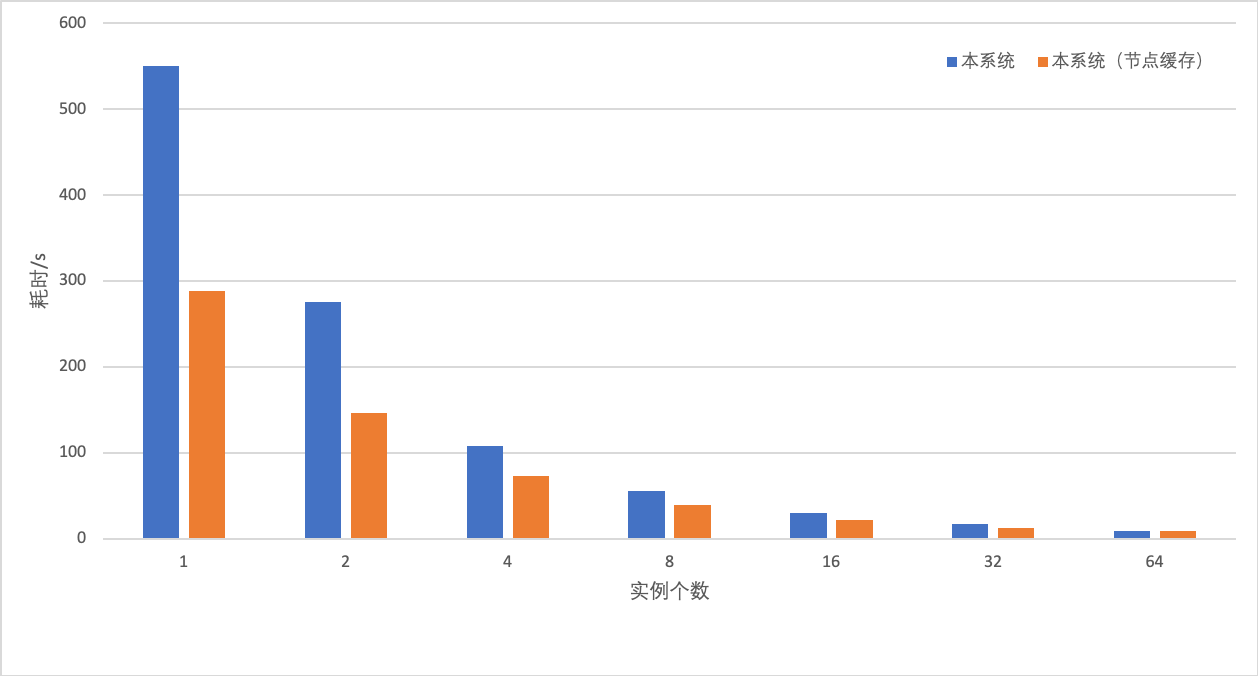
\includegraphics[width=12cm]{images/minstances.png}
    \caption{多实例千次运行耗时}
    \label{fig:minstantces}
\end{figure}


从可拓展性测试中可以看出,多实例可以规避系统整体运行时间受到单个模型最大运行时间影响的限制。

如图\ref{fig:minstantces}所示,随着集群中实例数的增加,完成1000次诊断的时间也在不断减少:
相比一个实例,在把实例数增加到64个之后,完成1000次面诊时间可以从500多秒下降到8秒左右。
在应对大批量用户的场景时,可以通过增加系统的硬件资源来满足用户的需求。

\section{本章小结}

本章分别介绍了利用面诊系统进行的两个交互实验,两个实验分别介绍了实验的设计和实验的结果。
通过分析实验结果,本文发现本文提出的增加系统可用性的设计能够提高用户的交互体验;在可解释设计的实验过程中,本文发现对和健康相关的权重进行解释时,柱状图会引起用户的反感和恐慌,而雷达图能够避免出现这一情况。
总的来说,增加系统的可解释性,对系统中的概念和结果进行解释,能够提高用户对结果的理解程度和对系统的信赖程度。


